% !TEX program = xelatex
\documentclass[a4paper]{exam}
\usepackage{amsmath}
\usepackage{amsthm}
\usepackage[left=1.8cm,right=1.8cm,top=2.2cm,bottom=2.0cm]{geometry}
\usepackage[UTF8]{ctex}
\usepackage{enumerate}
\usepackage{fancyhdr}
\usepackage{xpatch}
\usepackage{graphicx} 
\usepackage{float} 
\usepackage{subfigure} 
\usepackage{amsfonts}
\usepackage{mathtools}
\usepackage{framed}
\usepackage{multicol}
\usepackage{minted}
\usepackage{fontspec}
\usepackage{float}
\usepackage{tikz}
\usepackage{multicol,comment}
\usepackage{biblatex}
\addbibresource{01-discussion.bib}
\usepackage[section]{placeins}
\makeatletter

\newcommand{\answerprompt}[1][\textbf{Answer:}]{#1}

\noprintanswers


\AtBeginDocument{\xpatchcmd{\@thm}{\thm@headpunct{.}}{\thm@headpunct{}}{}{}}
\makeatother

\pagestyle{fancy}
\renewcommand{\baselinestretch}{1.15}
\newcommand{\code}[1]{\texttt{#1}}
\usepackage{paralist}
\let\itemize\compactitem
\let\enditemize\endcompactitem
\let\enumerate\compactenum
\let\endenumerate\endcompactenum
\let\description\compactdesc
\let\enddescription\endcompactdesc

% shorten footnote rule
\xpatchcmd\footnoterule
  {.4\columnwidth}
  {1in}
  {}{\fail}

\title{CS 131 Compilers: Discussion 1: Lexical Analysis}
\author{\textbf{杨易为}~~\textbf{吴凌云}~~\textbf{樊雨鑫} \\ \texttt{ \{yangyw,wuly2,fanyx\}@shanghaitech.edu.cn}}



\begin{document}
\maketitle
\section{Welcome to the Compiler's World}
\subsection{Some General Views}

We've covered in class that the compiler includes lexical analysis, in which we get tokens. This process is called the scanner of the program.
\begin{center}
  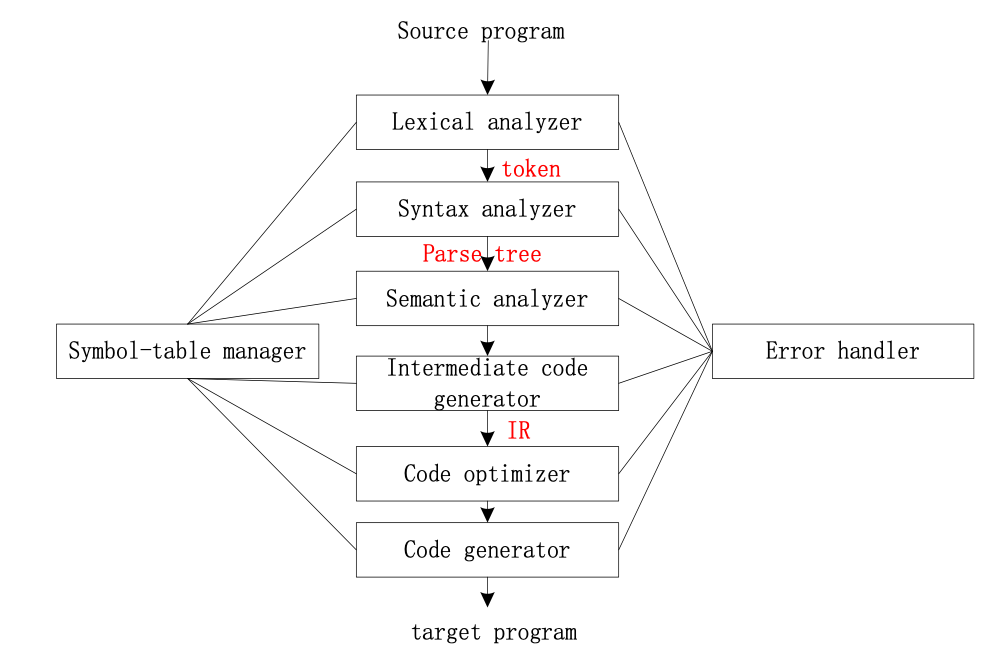
\includegraphics[height=6cm]{img/01-phases.png}
\end{center}

To make a detailed definition of compiling a program into a machine recognizable text and discuss whether kind of language is readable by a Turing Machine or so-called computer, we introduce regular expressions. Formally, we have Kleene closure and positive closure of a language to describe a language. Then NFA, DFA, DFA minimization are tools to accept the language. Regex has some limitation in describing a language and how to evaluate its power of it? Context Free Grammer is introduced and its solution LL Parsing and LR Parsing.

Till now, we have made the program into an Intermediate Representations, which in our project is Abstract Syntax Tree. We'll then make some type checking on it. This takes into the definition of Operational Semantics. For a modern languages like LLVM or those who compiled into LLVM IR, they have Intermediate Representations where passes can be cast on to optimize the code. Those optimizations are basically machine unrelated. Other intermediate representations include 3 address code and Single Static Code. Some of them are more low level and others are very similar to the AST, which depends on how heavy the analysis and the optimization can be cast on. We'll cover intra-basic-block optimization, dataflow analysis, security problems like Control Hijacking attacks. Language may allocate resources on stack or heap, we can do runtime garbage collections to make the resources reallocatable.

The eventual process of a compiler is Code Generator to generate machine code, we'll cover transforming the IR into the RISC-V backend that we've covered in Computer Architecture classes. Wish you good luck in the Compiler class.

\subsection{Why Both Parser and Lexer?}
Only lexers in dealing with the C++ code do not deal with nested grammar. The well-defined C++ code is even not acceptable by the modern parser.

In the old compiler, We don't recognize \code{vector<vector<> >}. For example \code{vector<vector<int> > v}, some compiler will compile into \code{vector < vector < int >> v}. Other than that, we have Most vexing parse.

\begin{figure}[H]
  \begin{minted}[mathescape, linenos]{c}
struct Timer {};
struct TimeKeeper {
  explicit TimeKeeper(Timer t);
  int get_time();
};
int main() {
  TimeKeeper time_keeper(Timer());
  return time_keeper.get_time();
}
    \end{minted}
\end{figure}

TimeKeeper time\_keeper(Timer()); is ambiguous, since it could be interpreted either as a variable definition for variable time\_keeper of class TimeKeeper, initialized with an anonymous instance of class Timer or a function declaration for a function time\_keeper that returns an object of type TimeKeeper and has a single (unnamed) parameter, whose type is a (pointer to a) function[Note 1] taking no input and returning Timer objects. \cite{mvp}

Julia is language with no Lexer and with parser, its parser reads from the string stream to generate the AST. It makes a lot of Context-Sensitive keywords and grammar struct which is difficult to formally describe, functional language's manual is shorter than languages like C++. But we can see that only parser is actually possible to parse the code. The lexer to decide the token is for sake of speed. But Lex/Yacc is fast enough to take over the speed. In Julia, operator and token are the same. \code{import Base.*} means import operator* from class Base, also means import all subclasses in class Base.

Thus mere lexer and mere parser are not wise.
\subsection{How can a simple regex work in your project?}
\begin{enumerate}
  \item Any Search with Regex option.
  \item You can write a plugin for a new language like Julia to support highlighting in vim/vscode/jetbrains.
\end{enumerate}
\subsection{Stages of Compilations}
\subsubsection{Convert the C++ source code into a sequence of tokens.}
Compilers are conceptually broken down into multiple phases, each of which carries out transformations on a source program towards the compiler’s ultimate goal; the gener-ation of a target program.  The result of each phase is an intermediate representationthat facilitates the implementation of subsequent phases (or,  if it is the last phase,the result is the target program). The first phase in a compiler, the lexical analyzer or lexer, reads an input stream of characters and converts it into a stream oftokensto be sent to the parser for syntactic analysis.

\begin{figure}[H]
  \begin{minted}[mathescape, linenos]{c}
// n! = 1 * 2 * 3 * .... * (n-1) * n
int factorial(int n) {
    int result = 1;
    for(int i = 2; i <= n; i++)
        result *= i;
    return result;
    }
    \end{minted}
\end{figure}

\begin{solution}
  KEYWORD ("public") KEYWORD ("static") KEYWORD ("int") ID("factorial") LPAREN KEYWORD ("int") ID ("n") RPAREN LCURLY KEYWORD ("int") ID ("result") ASSIGN INTLIT("1") SEMI FOR LPAR KEYWORD("int") ID("i") ASSIGN INTLIT("2") SEMI ID ("i") LEQ ID ("n") SEMI ID("i") OP("++") RPAREN ID("result") OP(*=) ID ("i") SEMI KEYWORD ("return") ID ("result") SEMI RCURLY
\end{solution}
\subsubsection{The rest of the compilations.}
What are the rest of the stages of compilation? List them in order and write a brief description about what they and what they take as input and what they output.\\

\begin{solution}
  \begin{enumerate}
    \item Parsing: Takes in a stream tokens, outputs an abstract syntax tree (AST), and checks to make sure the program is syntactically correct (matching parentheses, well-formed expressions, etc.)
    \item Semantic Analysis: Takes in an AST, and makes sure the program makes sense semantically, does type checking as well. Returns a decorated AST (with the corresponding types of variables/expressions/etc. or a IR (intermediate representation) for optimization.
    \item (Optional) Optimization: Takes in an AST or an IR, and generates an optimized AST or IR.
    \item Code generation: Takes in an AST or IR and generates code for the specific backend which this compiler is targetting.
    \item (Optional) Optimization: Takes in the backend code and performs optimizations on that, leaving optimized back-end code.
    \item \begin{enumerate}
            \item Executable generation: Takes in assembly files, assembles them into object files, and links object files to form an executable.
            \item Virtual Machine: Can interpret VM IR code or a decorated AST.
          \end{enumerate}
  \end{enumerate}
\end{solution}



\section{Regular Expressions}
The lexer needs to scan and identify finite character sequences that match a pattern corresponding to a particular token (the matching strings are also called lexemes). Patterns of finite strings can be codified using regular expressions, each of which specifies what is called a regular language. Kleene’s theorem states that any regular language can be recognized by a finite state automaton (FSA) and any language that is recognized by an FSA is regular.


\subsection{What language is denoted by each of the following regular expressions?}
Try to writing down a few simple strings and give a concise description of the language.

\subsubsection{[a-zA-Z][a-zA-Z0-9]$*$}

\begin{solution}
  Identifiers
\end{solution}
\subsubsection{$((\epsilon\mid a)b*)*$}
\begin{solution}
  All strings containing a and b characters, including the empty string. Simplified: $[\mathrm{ab}] *$
\end{solution}
\subsection{Write a regular expression for the following languages.}
\subsubsection{Uppercase Letters}
{All strings of uppercase letters, where the letters are in ascending lexicographic order (empty string allowed).}
\begin{solution}
  $A * B * \ldots . Z *$
\end{solution}
\subsubsection{ShanghaiTech Teacher's email addreess}
{xxxx@shanghaitech.edu.cn}, different error handler for different inputs? Suppose you have a large spreadsheet, each row of which has a firstname,lastname,and email column.  You want to find all people who use an email address of the form firstname+lastname@shanghaitech.edu.cn.   Write  a  regular  expression  using  backreferences that describes this pattern.
\begin{solution}
  $(\backslash p\{L\}+),(\backslash p\{L\}+),([0-9]*) \backslash 1 \backslash+\backslash 2+\backslash 3 @shanghaitech.edu.cn$
\end{solution}

\subsubsection{Months and Dates}
The following four strings: October 8th, October 8, Oct 8th, Oct 8 (Be as concise as possible with your regex)

\begin{solution}
  Oct (ober)? $\ $ s8 (th)?
\end{solution}

\subsubsection{Ones and Zeros}
Even binary numbers without leading 0.
\begin{solution}
  $1[01] * 0 \mid 0$
\end{solution}
\subsubsection{Ones and Zeros Plus}
Binary sequence that can be divided by 5 without remains.
\begin{figure}[h]
  \centering
  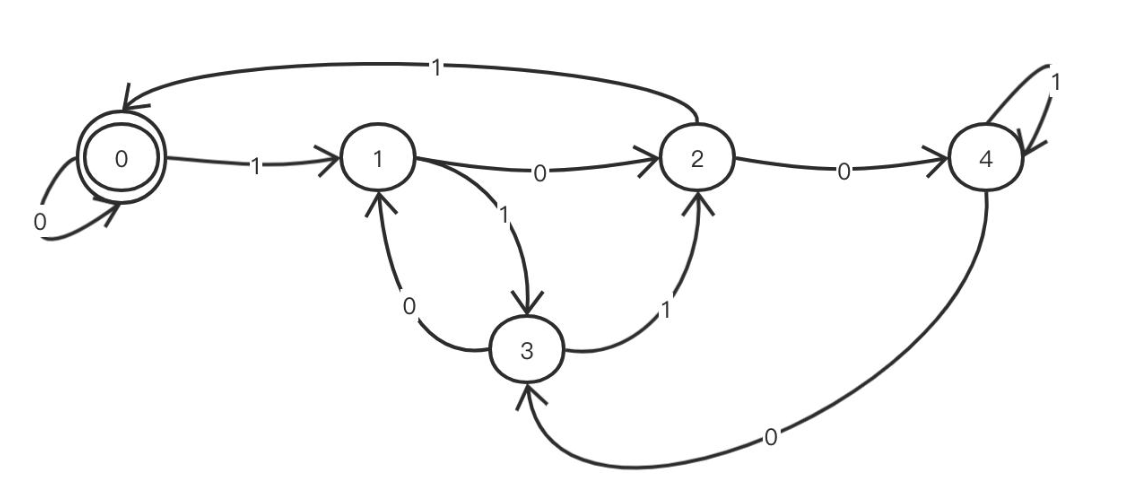
\includegraphics[width=\linewidth]{./img/leading_five.png}
  \caption{LeetCode 1018. Binary Prefix Divisible By 5}
\end{figure}
\begin{solution}
  \begin{enumerate}
    \item How many state should the Autometa have? mod 5: $5 .$
    \item What's the transmission function? think like DP. (小学奥数)
          \item\begin{enumerate} \item The (current state $^{*} 2+$ the last digit of the binary) $\% 5$
            \item The current bit is to tell which number $\bmod 5=0 / 1 / 2 / 3 / 4$
            \item The rest is very easy to calculate.
          \end{enumerate}\end{enumerate}

  DFA to RE refer to \cite{dfatoregex}.
\end{solution}

\printbibliography

\end{document}
